
\section{Sort profiles and normalization candidates}
\label{sec:profiles}

Throughout this section the pure type specification is finite and every
legal expression is weakly normalizing for full beta reduction. We use
the substitution, generation, context-conversion, subject-reduction and
confluence properties established in the preliminaries. Write $M^\#$
for the normal form of a legal expression, up to alpha conversion.
In particular, the expected type of a judgment has a normal form: it is
either sorted or already a literal sort. No uniqueness of sorts or
product rules is assumed.

We first associate a finite set of sorts to each type. These sets will
order the normalization argument. Within one part of that order we
shall construct sets of terms that pass certain application tests. The
main result of the section is an interface theorem: any construction
with the specified substitution and product properties advances the
normalization argument by one component.

\subsection{Profiles and the dependency graph}

For a sort $s$ and sets of sorts $I,J$, put
\[
 \operatorname{Ax}(s)=\{t:(s,t)\in\mathcal A\},\qquad
 \operatorname{Out}(I,J)
 =\{c:\text{some }a\in I,\ b\in J\text{ satisfy }(a,b,c)\in\mathcal R\}.
\]
For an expected type $T$ in a valid context $\Gamma$, define its
\emph{profile} by
\[
             \pi_\Gamma(T)=\{s:\Gamma\vdash T^\#:s\}.
\]
The profile can be empty when $T$ is an unsorted literal sort. When the
context is clear we omit its subscript. A \emph{neutral expression} is
a variable followed by zero or more arguments.

\begin{lemma}[Normal profiles]
\label{lem:normal-profiles}
A sorted normal expression is a sort, a neutral expression, or a
product. Its profile is determined as follows:
\begin{enumerate}
\item a literal sort $s$ has profile $\operatorname{Ax}(s)$;
\item a neutral expression has a singleton profile $\{s\}$, and
      $\operatorname{Ax}(s)$ is nonempty;
\item a normal product $\Pi x:D.E$ has profile
\[
 \operatorname{Out}\bigl(\pi_\Gamma(D),
                         \pi_{\Gamma,x:D}(E)\bigr).
\]
\end{enumerate}
Profiles are unchanged by valid thinning and context conversion.
If $\xi:\Gamma\to\Delta$ is a typed substitution, then
\begin{equation}
                  \pi_\Gamma(T)
                    \subseteq\pi_\Delta(T\xi).
\label{eq:profile-growth}
\end{equation}
\end{lemma}

\begin{proof}
A normal application is variable-headed: a lambda head would be a
redex, and a sort or product cannot have a product type by generation
and product compatibility. A lambda cannot have a literal sort type
for the same reason. Generation for a sort gives exactly its axiom
targets. Generation and product formation give the two inclusions in
the formula for a product, separately for every applicable rule.

For a neutral expression, its type is unique up to conversion. Indeed,
the assertion for its head variable follows from its declaration.
Inductively, generation and compatibility of convertible products
identify the domain and instantiated codomain at each further
application. Thus two literal sort types of a neutral are identical.
Its literal sort type $s$ is itself sorted. For a lone variable its
declaration type is sorted and convertible to $s$; confluence makes
that declaration type reduce to $s$, and subject reduction sorts $s$.
For a nonempty application spine, correctness of the expected type
already gives a sorting of $s$. Generation for $s$ now implies
$\operatorname{Ax}(s)\ne\varnothing$.

Thinning preserves the profile by induction on normal syntax. At a
neutral, an existing sort is retained and uniqueness excludes any new
one. At a product apply the induction also in its extended binder
context. Literal sorts do not depend on the context. Context conversion
preserves all relevant judgments in both directions, hence preserves
profiles as well.

Finally, if $s\in\pi_\Gamma(T)$, substitution gives
$\Delta\vdash T^\#\xi:s$. Reduction of $T$ to $T^\#$ commutes with
substitution, so $T^\#\xi$ and $T\xi$ have the same normal form.
Subject reduction therefore gives
$\Delta\vdash(T\xi)^\#:s$. This proves the inclusion. For a
substituted product the outer product persists, and its components
normalize separately; context conversion transports the open
codomain to the normalized domain. The same inclusion consequently
holds at corresponding product children.
\end{proof}

A nonempty profile is \emph{feasible} if it occurs in some valid
context. Since the specification is finite, there are only finitely
many feasible profiles.

\begin{lemma}[Feasible profiles]
\label{lem:feasible-profiles}
The feasible profiles form the smallest family containing
\[
 \operatorname{Ax}(s)\quad\hbox{and}\quad\{s\}
       \qquad\bigl(\operatorname{Ax}(s)\ne\varnothing\bigr)
\]
and closed under nonempty values of $\operatorname{Out}$.
\end{lemma}

\begin{proof}
Necessity follows by induction on a sorted normal expression, using
Lemma~\ref{lem:normal-profiles}. Conversely, $s$ witnesses
$\operatorname{Ax}(s)$, and a variable declared at type $s$ witnesses
$\{s\}$. Given normal witnesses for $I$ and $J$, rename their finite
contexts apart and combine those contexts by thinning. Form a product
with the first witness as domain and the second as a codomain
independent of its fresh binder. Its profile is exactly
$\operatorname{Out}(I,J)$. These witnesses are normal.
\end{proof}

Call $(I,J,K)$ a \emph{profile triple} when $I,J,K$ are feasible and
$K=\operatorname{Out}(I,J)$. Define the \emph{primary graph}, a finite signed directed graph on
the feasible profiles, by adding:
\begin{itemize}
\item a positive edge $L\to J$ whenever $L\supsetneq J$;
\item for each profile triple $(I,J,K)$, a negative edge $I\to K$
      and a positive edge $J\to K$.
\end{itemize}
Parallel edges retain their signs and their associated triples. Here and
below a path means a finite directed walk: vertices and edges may repeat.
Its parity is the parity of its number of negative edges; a
length-zero path is even.

If $T=\Pi x:D.E$ has profile $K$, write $I=\pi(D)$ and
$J=\pi(E)$. For every typed $n:D$, profile growth gives
\begin{equation}
 L=\pi\bigl((E[x:=n])^\#\bigr)\supseteq J,
 \qquad L\longrightarrow J\longrightarrow K
 \quad\hbox{by positive edges},
\label{eq:codomain-ascent}
\end{equation}
where the first edge is omitted when $L=J$.

\begin{figure}[ht]
\centering
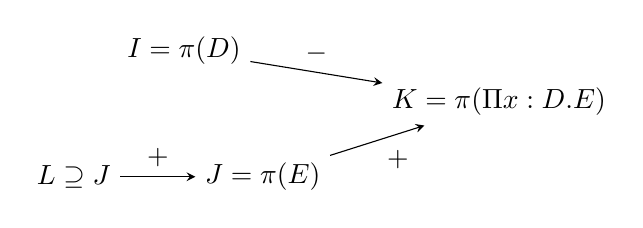
\begin{tikzpicture}[>=stealth,baseline=(current bounding box.center)]
\node (I) at (0,1.1) {$I=\pi(D)$};
\node (L) at (-1.4,-.5) {$L\supseteq J$};
\node (J) at (1,-.5) {$J=\pi(E)$};
\node (K) at (4,.45) {$K=\pi(\Pi x:D.E)$};
\draw[->] (I) -- node[above] {$-$} (K);
\draw[->] (J) -- node[below right] {$+$} (K);
\draw[->] (L) -- node[above] {$+$} (J);
\end{tikzpicture}
\caption{The domain and open codomain point to their product. An
instantiated codomain has profile $L\supseteq J$ and also has a
positive path to the product. The edge $L\to J$ is omitted if $L=J$.}
\label{fig:profile-dependencies}
\end{figure}

Order the strongly connected components so that every predecessor
component is processed first. At a given stage let $S$ be the current
component and $U$ the union of the already processed components.
Thus $U$ is predecessor-closed, and every predecessor of $S$ lies in
$U\cup S$. The graph immediately gives the following facts:
\begin{enumerate}
\item the domain and open codomain of an $S$ product have profiles
      in $U\cup S$;
\item every instantiated codomain of that product has profile in
      $U\cup S$;
\item any feasible enlargement of a profile in $S$ lies in $U\cup S$;
\item any feasible enlargement of a profile in $U$ lies in $U$.
\end{enumerate}
All statements also hold after valid thinning or context conversion.

\subsection{Application tests and candidates}

Use the saturated context $\Omega$ from the preliminaries. A judgment
over $\Omega$ means a judgment over some finite prefix; finitely many
judgments may always be thinned to a common prefix. Profile invariance
makes their profiles independent of this choice. An \emph{actual
type} is a normal sorted expression over $\Omega$, or a literal sort.
For such a type put
\[
 \operatorname{Ty}(T)=\{h:\Omega\vdash h:T\},\qquad
 \top_T=\operatorname{Ty}(T)\cap\operatorname{SN}_\beta.
\]
Here and below strong normalization includes reduction in annotations.

A \emph{tested stack at $T$} is a finite list defined inductively.
The empty list is always a tested stack. If $T=\Pi x:D.E$,
$n\in\top_D$, and $\vec m$ is a tested stack at
\[
                     T_n=(E[x:=n])^\#,
\]
then $(n,\vec m)$ is a tested stack at $T$. This definition follows
these exact successive types; it does not range over alternative
typings of a term. Define
\[
 G_T=\{h\in\operatorname{Ty}(T):
            h\,\vec n\in\operatorname{SN}_\beta
            \text{ for every tested stack }\vec n\text{ at }T\}.
\]
We shall establish, component by component, the invariant
\begin{equation}
                    G_T=\top_T\qquad(\pi(T)\in U).
\label{eq:processed-invariant}
\end{equation}

\begin{lemma}[Elementary properties of the tests]
\label{lem:test-properties}
For every actual type $T$, $G_T\subseteq\top_T$. If $T$ is a literal
sort, equality holds. Every variable typed at $T$ belongs to $G_T$.
If $T=\Pi x:D.E$, $h\in G_T$, and $n\in\top_D$, then
$h\,n\in G_{T_n}$.
\end{lemma}

\begin{proof}
The empty stack gives the inclusion; at a literal sort it is the only
stack. A variable followed by finitely many strongly normalizing
arguments is strongly normalizing: its head never contracts, and a
reduction decreases the sum of the arguments' reduction heights.
This proves the assertion for variables. For propagation, append any
tested stack at $T_n$ to $n$ and apply the definition of $G_T$.
Application and conversion give the required exact typing at $T_n$.
\end{proof}

\begin{lemma}[Head expansion for strong normalization]
\label{lem:sn-head-expansion}
Suppose that $D,P,n,m_1,\ldots,m_k$ are strongly normalizing and that
\[
                    P[x:=n]m_1\cdots m_k
\]
is strongly normalizing. Then
$(\lambda x:D.P)n m_1\cdots m_k$ is strongly normalizing.
\end{lemma}

\begin{proof}
Every strongly normalizing expression has a finite maximal reduction
length. Indeed, reduction is finitely branching; if lengths were
unbounded, at least one immediate reduct would again have unbounded
lengths, and iterating this choice would give an infinite reduction.
Write $\ell(Q)$ for this maximal length and induct on
\[
        \ell(D)+\ell(P)+\ell(n)+\sum_{i=1}^k\ell(m_i).
\]
The head reduct is strongly normalizing by hypothesis. Every other
immediate reduct changes one displayed component and strictly lowers
this sum. Its head contractum is either unchanged or is a reduct of
the old head contractum. For a step in $n$, contract the corresponding
step in each of its finitely many copies in $P[x:=n]$; there may be
zero copies. For a step in the annotation, the contractum is unchanged.
Thus the new contractum is strongly normalizing, and the induction
applies. Every immediate reduct is strongly normalizing, which proves
the claim.
\end{proof}

\begin{definition}[Candidate at an actual type]
\label{def:candidate}
A candidate at $T$ is a set $C$ satisfying
$G_T\subseteq C\subseteq\top_T$ and the following head-expansion
property: if
\[
 r=(\lambda x:D.P)n\,\vec m\in\operatorname{Ty}(T),
\]
all displayed components $D,P,n,\vec m$ are strongly normalizing, and
$P[x:=n]\vec m\in C$, then $r\in C$. Denote the candidates at $T$
by $\mathcal C(T)$.
\end{definition}

Reduction closure is not part of this definition. All subsequent
candidate arguments use only the properties just stated.
This is a local variant of the reducibility-candidate method
\cite[Chapters~6 and~14]{Girard1989}; the next lemma proves its required
lattice and product closure directly.

\begin{lemma}[Candidate lattice and product tests]
\label{lem:candidate-lattice}
The inclusion-ordered set $\mathcal C(T)$ is a complete lattice with
largest element $\top_T$. Write $\bot_T$ for its least element.
For an actual product $T=\Pi x:D.E$, choose a set
$A\subseteq\top_D$. For each $n\in A$ choose any family of candidates
$C_{n,a}\in\mathcal C(T_n)$ indexed by a set $Q_n$. Then
\begin{equation}
 \{h\in\top_T:\text{for every }n\in A\text{ and }a\in Q_n,
                                  \ h n\in C_{n,a}\}
\label{eq:product-test-candidate}
\end{equation}
is a candidate at $T$.
\end{lemma}

\begin{proof}
Lemma~\ref{lem:sn-head-expansion} shows that $\top_T$ is a candidate.
Intersections of candidates preserve all three requirements of
Definition~\ref{def:candidate}; take the empty intersection to be
$\top_T$. Therefore every family has a meet, and its join is the
intersection of its common upper bounds. This family of upper bounds
is nonempty because it contains $\top_T$. In particular, the least
candidate is the intersection of all candidates.

For \eqref{eq:product-test-candidate}, a term in $G_T$ passes every
test by Lemma~\ref{lem:test-properties} and the containment
$G_{T_n}\subseteq C_{n,a}$. Suppose a head contractum belongs to
\eqref{eq:product-test-candidate} and its expansion has strongly
normalizing components. Lemma~\ref{lem:sn-head-expansion} gives the
expansion's membership in $\top_T$. Append a prescribed $n\in A$ to
its spine. The enlarged head contractum lies in $C_{n,a}$ for every
$a$, and all enlarged components are strongly normalizing. Head
expansion in $C_{n,a}$ gives the required membership of the enlarged
spine. This proves every test, without using reduction closure of a
candidate.
\end{proof}

At profiles in $U$, the invariant
\eqref{eq:processed-invariant} forces every candidate to equal
$\top_T$. This is why previously processed types need no further
choices.

\subsection{The interface for one component}
\label{subsec:candidate-interface}

We now specify exactly what a component construction must supply.
The context $\Gamma$ and its syntax will be called \emph{generic};
a typed substitution $\xi:\Gamma\to\Omega$ supplies raw actual
images. An environment also contains auxiliary parameters $\theta$
for the declarations. Each construction below specifies their sets.
Require an empty parameter environment and compatible parameter
extensions along every typed context extension. Restrictions to
preceding declarations are understood when interpreting declaration
types.

For each normal generic expected type $T$ with
$\pi_\Gamma(T)\in S$, the construction supplies a candidate
\[
       R_{\Gamma,T}(\xi,\theta)
                     \in\mathcal C\bigl((T\xi)^\#\bigr).
\]
For any other normal generic expected type use the convention
\[
              R_{\Gamma,T}(\xi,\theta)=\top_{(T\xi)^\#}.
\]
When no ambiguity arises write simply $R_T$. Actual profiles obtained
from generic profiles in $S$ lie in $U\cup S$, and an actual profile
in $U$ makes the candidate equal to top.

The required properties are the following.
\begin{enumerate}
\item\label{item:interface-invariance}
\emph{Invariance.} Valid thinning, context conversion, and pointwise
convertible actual images preserve the candidates on old syntax when
the old parameters are unchanged. Capture-avoiding renaming of generic declared and bound variables preserves
the interpretation, with the substitution and parameter environment reindexed
on declared variables and all actual images and parameter values unchanged.

\item\label{item:interface-product}
\emph{Product equality.} Let $T=\Pi x:D.E$ have generic profile in
$S$ and actual profile in $S$. For each $n\in R_D$, specify a
nonempty collection $Q_{T,n}$ of compatible parameter extensions to
$\Gamma,x:D$ with substitution $\xi[x\mapsto n]$. Then $R_T$
equals the following product-test candidate. Its members are exactly
the $h\in\top_{(T\xi)^\#}$ such that, for every $n\in R_D$:
\begin{itemize}
\item if the actual type $(E(\xi[x\mapsto n]))^\#$ has profile
      in $S$, then $h n\in R_E(\xi[x\mapsto n],\theta')$ for
      every $\theta'\in Q_{T,n}$;
\item if that actual profile lies in $U$, then $h n$ is strongly
      normalizing at that exact normal type.
\end{itemize}
Application is well typed because the actual domain of the normal
product $(T\xi)^\#$ is $(D\xi)^\#$; substitution and normalization
identify its instantiated codomain with the displayed actual type.
The generic domain profile belongs to $U\cup S$, so $R_D$ is the
candidate supplied by the construction or the prescribed top in $U$.

\item\label{item:interface-specialization}
\emph{Specialization.} In the product situation, if
$\Gamma\vdash N:D$, $N\xi\in R_D$, and $h\in R_T$, then
\begin{equation}
          h(N\xi)\in
               R_{\Gamma,(E[x:=N])^\#}(\xi,\theta).
\label{eq:interface-specialization}
\end{equation}
It is enough to find one of the tested parameter extensions for which
the codomain candidate is contained in the candidate on the right.
If the actual codomain profile is in $U$, this follows directly from
the strong-normalization test.
\end{enumerate}
Both directions of the product-equality requirement are required: the lambda case uses its
introduction direction and application uses its elimination direction.

A typed environment $(\xi,\theta)$ is \emph{admissible} if, for each
declaration $x:B$ of $\Gamma$, its image satisfies the following
condition, evaluated over the preceding declarations:
\[
 \begin{cases}
 \xi(x)\in R_{B^\#},&\pi(B)\in S,\\
 \xi(x)\in\operatorname{SN}_\beta,&\pi(B)\in U,\\
 \xi(x)\in G_{(B\xi)^\#},&\pi(B)\notin U\cup S.
 \end{cases}
\]
The exact typings in these conditions follow from typed substitution
and conversion. Admissibility imposes no separate restriction on the
auxiliary parameters.

\begin{lemma}[Transport of strongly normalizing terms]
\label{lem:sn-fundamental}
Assume \eqref{eq:processed-invariant} and an implementation of
the three interface requirements in Section~\ref{subsec:candidate-interface}
for $S$. If $\Gamma\vdash M:A$, the expression $M$ is strongly
normalizing, and $(\xi,\theta)$ is admissible, then
\begin{equation}
                         M\xi\in R_{\Gamma,A^\#}(\xi,\theta).
\label{eq:sn-fundamental}
\end{equation}
\end{lemma}

\begin{proof}
Induct lexicographically on $(\ell(M),|M|)$, where $|M|$ is syntax
size including annotations. The induction is simultaneous over all
typings, contexts, and admissible environments. A proper subexpression
has no larger reduction height and smaller size; a beta reduct has
strictly smaller height. Typed substitution gives all required actual
typings throughout.

We shall repeatedly use a fresh-variable extension. If a binder has
raw generic annotation $B$, then $B\xi$ is sorted over a finite
prefix of $\Omega$. Saturation supplies a fresh variable $z$ declared
at that raw type, beyond a common prefix for the finite expressions
in question. Choose $z$ outside the free names of all other images.
It belongs to $G_{(B\xi)^\#}$ by
Lemma~\ref{lem:test-properties}, and hence satisfies whichever of
the three admissibility conditions applies. Any allowed parameter
extension can be used. Invariance retains the assumptions on old
variables. If the induction proves the body with $x$ sent to $z$
strongly normalizing, renaming $z$ back to a bound $x$ proves strong
normalization of the open substituted body.

For a sort, $M\xi=M$ is normal, and its expected normal type is a
literal sort. At a literal sort $G$ equals top, so this suffices for
membership in any candidate. For a product, apply the induction to
its domain and to its open codomain under a fresh-variable extension.
The two substituted components are strongly normalizing, so the
product is strongly normalizing. Its expected normal type is again
a literal sort, giving the conclusion.

Let $M=\lambda x:B.P$. The induction on $B$, and on $P$ under a
fresh-variable extension, proves strong normalization of the actual
annotation and open body. Hence $M\xi$ is strongly normalizing.
This already proves the conclusion unless both the generic and the
actual normalized expected types have profiles in $S$. In the latter
case write $A^\#=\Pi x:D.E$. Generation and product compatibility
identify $D$ with the normal form of $B$ and identify $E$ with the
normal body type, after context conversion under the binder.

Context-convert the generic body judgment to
$\Gamma,x:D\vdash P:E$. Take an arbitrary $n\in R_D$ and arbitrary
prescribed parameter extension in $Q_{A^\#,n}$. Convert $n$ to the
actualized type $D\xi$ and extend this context's substitution by
$x\mapsto n$. This is admissible:
the generic domain profile is in $U\cup S$, and the test condition is
exactly the required candidate or SN condition. Apply the induction
to the context-converted judgment for $P$ in this very extension.
It gives the required codomain candidate for the head contractum of
$(M\xi)n$. The actual annotation, open body and $n$ are strongly
normalizing. Head expansion in that codomain candidate proves the
test. If the actual codomain profile is in $U$, use any compatible
parameter extension, the body's strong normalization, and
Lemma~\ref{lem:sn-head-expansion}. We have verified every product
test; the introduction direction of
the product-equality requirement proves the conclusion.

For an application, inspect its entire left-associated spine. If its
head is a lambda, write
\[
                M=(\lambda x:B.P)N\,\vec L.
\]
Contract its first redex generically to $M'$. Subject reduction gives
$\Gamma\vdash M':A$ and $\ell(M')<\ell(M)$, so the induction gives
$M'\xi\in R_{A^\#}$. The components $B,P,N,\vec L$ are proper
subexpressions. Their inductions, using a fresh-variable extension for
the open $P$, give strong normalization of every component after
substitution. Substitution commutes with the displayed contraction up
to alpha conversion. Head expansion in $R_{A^\#}$ therefore proves
the result. This step does not invoke reduction closure of a candidate.

The remaining case is a neutral spine $xN_1\cdots N_k$, including
$k=0$. Starting at the normal form of the declaration type of $x$,
generation and neutral uniqueness determine its successive normal
expected types. Whenever a next argument occurs, the preceding type
is a product; convert that argument to its normalized domain and take
the normalized instantiated codomain as the next type. The induction
applied to each $N_i$ at this exact domain gives its candidate
membership and, in particular, strong normalization after substitution.
Typed substitution and confluence identify the actual successive
types with the normal forms of the corresponding generic types.

Track membership along the spine. A $G$ prefix propagates by
Lemma~\ref{lem:test-properties}. If the head declaration has profile
in $U$, admissibility and profile growth put it in actual top in $U$,
hence in $G$ by \eqref{eq:processed-invariant}. If a prefix has generic
profile in $S$, an actual profile in $U$ likewise gives $G$. Otherwise
its candidate product test applies to the next argument, and
\eqref{eq:interface-specialization} gives the next candidate. That
next generic profile lies in $U\cup S$ by the positive codomain path;
on reaching $U$ its membership is again in $G$. A head declaration
outside $U\cup S$ starts in $G$ by admissibility and requires no
further restriction on profiles. Thus the final prefix belongs either
to the desired candidate or to its subset $G$. No other spine head
can type as an application. This completes the induction.
\end{proof}

\begin{proposition}[Advancing one component]
\label{prop:advance-component}
Under the hypotheses of Lemma~\ref{lem:sn-fundamental},
\eqref{eq:processed-invariant} also holds for every actual type with
profile in $S$.
\end{proposition}

\begin{proof}
Fix $h\in\top_T$ with $\pi(T)\in S$ and any tested stack
$(n_1,\ldots,n_k)$ at $T$. Choose a common finite prefix $\Gamma$
of $\Omega$ supporting the relevant exact typings and use the
identity substitution. Choose parameters successively; all variable
images lie in $G$ and therefore the environment is admissible.
Apply Lemma~\ref{lem:sn-fundamental} separately to $h$ and to each
$n_i$ at its exact successive domain. Each is strongly normalizing
by hypothesis or by the definition of a tested stack.

Start with the resulting candidate membership of $h$ and iterate the
product tests and specialization along the stack. Each encountered
type has profile in $U\cup S$. In $S$ specialization supplies the
next candidate membership; in $U$ the invariant supplies $G$, which
propagates across every remaining frame. Thus $h n_1\cdots n_k$ is
strongly normalizing. The argument never assumes strong normalization
of an intermediate generic application and never applies the
fundamental lemma to such an application. Since the stack was
arbitrary, $h\in G_T$. The reverse inclusion is
Lemma~\ref{lem:test-properties}.
\end{proof}

\begin{proposition}[Completion of the interface argument]
\label{prop:interfaces-imply-sn}
If the interface can be implemented at every strongly connected
component, then every legal expression of the PTS is strongly
normalizing.
\end{proposition}

\begin{proof}
Process the finitely many components and apply
Proposition~\ref{prop:advance-component}. At the end, $G_T=\top_T$
for every actual type with nonempty profile. Empty-profile actual
types are literal sorts, for which this equality already holds by
Lemma~\ref{lem:test-properties}.

Suppose a typable expression is not strongly normalizing and choose
one of least syntax size, among all valid contexts and typings. Its
proper syntactic children are typable in the corresponding contexts,
including under binders, and so are strongly normalizing. A variable
or sort is normal; a product or lambda with strongly normalizing
children is strongly normalizing. The expression must therefore be
an application $f n$, with $f,n$ strongly normalizing. Generation
types $f$ at a product and $n$ at its domain. Normalize that product,
convert these typings, and embed the finite context into $\Omega$.
The resulting normal product is an actual type with nonempty profile:
it is sorted by correctness of types and cannot be a literal sort.
The equality $G_T=\top_T$ and its one-frame test now give strong
normalization of $f n$, a contradiction. This also handles an empty
feasible-profile graph, since the hypothetical application would
itself produce a feasible product profile.

Finally, every legal expression is typable by validity and correctness
of types, or is a literal sort. Literal sorts are normal. Hence the
conclusion holds with the full legal-expression and open-context scope.
\end{proof}

The remaining task is to construct the interface. We now do so in two
cases using only the profile graph. The other components require the
additional semantic construction developed later.

Figure~\ref{fig:component-contracts} separates the construction of an
interface from its use in the normalization induction. For the third
case, the observation construction has an additional graph hypothesis.
The typed obstruction proves that hypothesis from system-wide weak
normalization, independently of the candidate interpretation. Thus the
third branch, like the first two, supplies the full interface before
the processed invariant is advanced.

\begin{figure}[ht]
\centering
\begin{tikzpicture}[>=Stealth,
  contract/.style={draw,rounded corners,align=center,font=\small,
                   inner sep=6pt,text width=4.2cm}]
\node[contract,text width=11.8cm] (input) at (0,0)
  {Finite specification and system-wide weak normalization;\\
   current component $S$, processed predecessors $U$, and $G_T=\top_T$ on $U$};
\node[contract] (simple) at (-3.2,-2.25)
  {No odd closed walk, or no all-$S$ profile triple\\
   Propositions~\ref{prop:signed-component} and~\ref{prop:one-child-component}};
\node[contract] (remaining) at (3.2,-2.25)
  {Remaining components: observation construction and typed exclusion\\
   Propositions~\ref{obs:interface-theorem} and~\ref{prop:enc-exclusion}};
\node[contract,text width=10.7cm] (interface) at (0,-4.25)
  {Candidate interface for $S$ (Section~\ref{subsec:candidate-interface}):\\
   invariance, product equality in both directions, and specialization};
\node[contract,text width=10.7cm] (advance) at (0,-5.85)
  {$G_T=\top_T$ also on $S$ (Proposition~\ref{prop:advance-component});\\
   after all components, strong normalization (Proposition~\ref{prop:interfaces-imply-sn})};
\draw (input.south) -- (0,-.95);
\draw[->] (0,-.95) -| (simple.north);
\draw[->] (0,-.95) -| (remaining.north);
\draw (simple.south) -- (-3.2,-3.45) -- (0,-3.45);
\draw (remaining.south) -- (3.2,-3.45) -- (0,-3.45);
\draw[->] (0,-3.45) -- (interface.north);
\draw[->] (interface) -- (advance);
\end{tikzpicture}
\caption{The contracts of one component step. The right branch combines
the conditional observation construction with the independent proof of
its graph hypothesis. The arrows to the interface assert the complete
three-part contract, before any use of component advancement.}
\label{fig:component-contracts}
\end{figure}
\FloatBarrier

\section{Two component constructions}
\label{sec:simple-components}

Keep a current component $S$ and the invariant on its processed
predecessors $U$. The first construction uses signs to compensate for
the opposite variances of domain and codomain. The second uses a
single chain in each normal type when its two product children cannot
both remain in $S$.

\subsection{Components without an odd closed walk}

\begin{proposition}[The signed fixed-point construction]
\label{prop:signed-component}
If $S$ has no odd closed walk, it admits the candidate interface.
\end{proposition}

\begin{proof}
Choose a vertex of $S$. Assign to each vertex the parity of any path
from the chosen vertex to it. This is well defined: append a return
path to two proposed paths; different parities would produce an odd
closed walk. Give even vertices sign $+$ and odd vertices sign $-$.
Every internal positive edge preserves sign, and every internal
negative edge reverses sign.

Let $\mathcal T_S$ be the set of actual types with profile in $S$.
It is a set, since these are finite syntax over the countable context
$\Omega$. On
\[
                      \mathcal L=
                  \prod_{T\in\mathcal T_S}\mathcal C(T)
\]
use inclusion in coordinates with sign $+$ and reverse inclusion in
coordinates with sign $-$. This is a complete lattice by
Lemma~\ref{lem:candidate-lattice}. Extend a vector $v$ to actual
types in $U$ by $v_T=\top_T$.

Define an operator $F:\mathcal L\to\mathcal L$. At a nonproduct
type set $F(v)_T=\top_T$. At $T=\Pi x:D.E$, let
\[
 F(v)_T=\{h\in\top_T:\text{for every }n\in v_D,
                                      \ h n\in v_{(E[x:=n])^\#}\}.
\]
All indices belong to $U\cup S$ by the dependency graph, and this
is a candidate by Lemma~\ref{lem:candidate-lattice}.

The operator is monotone in the mixed order. In the usual inclusion
order its product clause is antitone in the domain coordinate and
monotone in every instantiated-codomain coordinate. An internal domain
has the opposite sign to $T$ by its negative edge. An instantiated
codomain in $S$ has the same sign as $T$ by its positive path through
the open codomain: the intermediate vertex must also lie in $S$,
since a vertex in $U$ has all its predecessors in $U$. Coordinates
in $U$ are constant. These observations
give exactly the required coordinatewise monotonicity, in either sign
of the output.

Tarski's fixed-point theorem \cite[Theorem~1]{Tarski1955} gives a fixed
point. We recall its short existence proof, which needs no continuity
assumption. Let $a$ be the supremum of all
$v$ satisfying $v\le F(v)$. For every such $v$, monotonicity gives
$v\le F(v)\le F(a)$, so $a\le F(a)$. Then
$F(a)\le F(F(a))$, making $F(a)$ one of the elements whose supremum
is $a$; hence $F(a)\le a$. Fix such a vector $a$.

No auxiliary parameters are needed. For a generic normal type $T$
with profile in $S$, define $R_T=a_{(T\xi)^\#}$ if its actual
profile is in $S$, and top otherwise. At a generic product with
actual profile in $S$, its actual normalized domain and all actual
instantiated codomains are exactly the indices in the operator clause.
Thus the fixed-point equality gives the required product equality,
with the unique parameter extension.

The actual normalized type determines the candidate, so thinning,
context conversion and pointwise convertible images preserve it.
For specialization the two actual type expressions
\[
 E(\xi[x\mapsto N\xi])
       \quad\hbox{and}\quad ((E[x:=N])^\#)\xi
\]
are convertible by substitution composition and normalization.
Their normal forms are identical. The two candidates are consequently
equal when that profile is in $S$, and both are top in $U$. A generic
child in $U$ remains there under substitution, so no additional case
arises. This proves all interface requirements.
\end{proof}

\subsection{Components with at most one internal product child}

Suppose now that there is no profile triple $(I,J,K)$ with
$I,J,K\in S$. For a normal type $T$ of profile in $S$, start at its
root. At a product continue to its child of profile in $S$, if it has
one; there is at most one. Stop at a nonproduct or at a product with
no such child. This is a finite path in the syntax tree.

If the path ends at a neutral expression whose head $y$ is free in
the starting context of $T$, define the \emph{support} of $T$ to be
$y$. Define its \emph{polarity} to be $+$ or $-$ according to whether
the path takes an even or odd number of domain steps. In every other
case the support is empty. Also declare support empty at a generic
profile outside $S$. In particular a head bound strictly inside
$T$ is not its support. The support of a codomain, considered in its
own extended context, may of course be its immediately preceding
binder.

Assign each declaration of a generic context a bit $0$ or $1$;
these are the parameters $\theta$. At a neutral we use the candidate
extremum selected by its head's bit, with $0$ selecting bottom and $1$
selecting top. Define candidates recursively on normal generic types
as follows. At an actual profile in $U$ use top. At a generic profile
outside $S$ also use top, as in the interface. Otherwise:
\begin{itemize}
\item at a sort use top;
\item at a neutral with head $y$ use
      $\bot_{(T\xi)^\#}$ or $\top_{(T\xi)^\#}$ according to
      $\theta(y)$;
\item at a product $T=\Pi x:D.E$ use the product-test candidate
      in Section~\ref{subsec:candidate-interface}. There is one prescribed
      bit for $x$: use $0$ if the support of $E$ is $x$ with positive
      polarity, $1$ if it is $x$ with negative polarity, and $1$ if
      $x$ is not supported. If $E$ has profile in $U$, its bit is
      irrelevant and we again choose $1$.
\end{itemize}
Every recursive child is smaller syntax; candidate existence follows
from Lemma~\ref{lem:candidate-lattice}. Context variables can always
be assigned bits, and the prescribed extension is nonempty.

\begin{lemma}[Dependence on support]
\label{lem:support-dependence}
For fixed typed actual images, the candidate of an $S$ type depends
on the bits of its starting context only through its support, if any.
Valid thinning and context conversion preserve the support, its
polarity, and the candidates. Pointwise convertible actual images
preserve the candidates when old bits agree.
\end{lemma}

\begin{proof}
Induct on the normal type. Sorts and actual-$U$ cases do not use
bits. A neutral uses only its head bit. At a product, any child in
$U$ is interpreted as top; only the unique $S$ child can depend on
old bits. Its support is propagated to the parent unless it is the
product's own binder, whose bit is fixed by the displayed rule.
This proves the dependence assertion. Profile invariance preserves
the same product path and its domain parity under thinning and
context conversion. In those operations and under convertible images,
the actual normal types agree. The recursive product tests then have
identical domains, codomains and prescribed bits, proving the stated
invariances.
\end{proof}

Use the notation $A\preceq_+B$ for $A\subseteq B$ and
$A\preceq_-B$ for $A\supseteq B$. Regard signs as $+1$ and $-1$
when multiplying them.

\begin{lemma}[Comparison after generic substitution]
\label{lem:support-substitution}
Let $\Gamma,y:B,\Delta$ be valid, let $\Gamma\vdash N:B$, and
let $T$ be a normal type of profile in $S$ in that context. Put
\[
 \Gamma'=\Gamma,\Delta[y:=N],\qquad
                         T'=(T[y:=N])^\#.
\]
Take typed substitutions of the two contexts into $\Omega$ whose
images are compatible with composition: the pre-substitution image
of $y$ is convertible to the actual image of $N$, and the other
images agree up to conversion. Equip the substitutions with bits
$\theta,\theta'$. Fix a comparison sign $\delta\in\{+,-\}$ and
assume:
\begin{enumerate}
\item the bits agree on any variable supported by both $T$ and $T'$;
\item if $y$ supports $T$ with polarity $\varepsilon$, then its
      pre-substitution bit is $0$ when $\delta\varepsilon=+$ and
      $1$ when $\delta\varepsilon=-$.
\end{enumerate}
Then, at their common actual normal type,
\[
             R_T(\xi,\theta)
                  \preceq_\delta R_{T'}(\xi',\theta').
\]
\end{lemma}

\begin{proof}
Induct on the pre-substitution syntax of $T$. The actual normal
types agree by substitution composition and confluence. If their
profile lies in $U$, both candidates are top. Otherwise that profile
lies in $S$, and so does the generic profile of $T'$: profile growth
puts it in $U\cup S$, and a generic profile in $U$ could only have
actual profile in $U$.

A sort is unchanged. A neutral whose head is not $y$ remains a
neutral with the same head after substitution and normalization; if
its actual profile is in $S$, the supported head is common and its
bit agrees. At a neutral headed by $y$, its polarity is positive and
the prescribed bit chooses the least candidate for forward inclusion,
or the greatest candidate for reverse inclusion. This compares it
with every possible candidate of $T'$. In particular we do not
recurse into the possibly larger normal expression obtained by
substituting for $y$.

Let $T=\Pi x:D.E$, choosing $x$ fresh for $N$ and for the
substitution data. The post-substitution type is again a product,
with its two substituted components normalized. Context-convert the
open codomain to the normalized post domain. To compare the product
test candidates in direction $\delta$, compare their domain
candidates in direction $-\delta$. On each common test compare their
codomain candidates in direction $\delta$, extending the actual
images by that same raw test and using the respective prescribed
bits for $x$. For example, for forward inclusion every post domain
test must be a pre domain test, and its pre codomain candidate must
be contained in its post codomain candidate.

If a pre child is in $U$, its generic substitute remains in $U$ and
both actual child candidates are top. If its generic substitute
grows into $U$, the common actual child profile is again in $U$,
with the same conclusion. In all other required child comparisons,
both generic child profiles are in $S$. Such a post child must be
the same unique $S$ child as before substitution: a pre off-path
child in $U$ cannot grow into $S$. Every common supported variable
other than the new binder $x$ therefore inherits the agreement
condition from the parent. If $y$ supports the child, the prescribed
extremum condition is also inherited: a domain step reverses both
the comparison direction and the support polarity, and a codomain
step reverses neither.

It remains to check the bits of $x$ when it is supported in both
open codomains. The pre support path ends at a neutral with head
$x$, which substitution for $y$ cannot change. Every product on
that path persists. The post support path must follow the same
positions: a pre off-path child remains in $U$, while truncation
of the path into $U$ would prevent the post codomain from being
supported by $x$. Thus both paths have the same number of domain
steps, their polarities agree, and the prescribed bits of $x$
agree. If substitution exposes $x$ through a neutral headed by
$y$, that portion of the induction instead stops at the extremum
case already proved; it imposes no further shared-support condition.

All hypotheses of the child inductions now hold. Their inclusions
give the desired product inclusion by the universal test definition,
in either direction. This completes the induction.
\end{proof}

\begin{proposition}[The one-child construction]
\label{prop:one-child-component}
If no profile triple has all three vertices in $S$, then the
bit-parametrized candidates above implement the candidate interface.
\end{proposition}

\begin{proof}
Candidate existence and product equality follow from the recursion.
Lemma~\ref{lem:support-dependence} gives the required invariances.
To verify specialization, let
$T=\Pi x:D.E$, take $\Gamma\vdash N:D$ with $N\xi\in R_D$,
and let $h\in R_T$. Its product test gives
\[
 h(N\xi)\in R_E(\xi[x\mapsto N\xi],\theta_x)
\]
when the actual codomain profile lies in $S$; here $\theta_x$ is
the prescribed binder extension. Apply
Lemma~\ref{lem:support-substitution} to substitution for $x$ in
$E$, with comparison direction $+$. All old bits agree. The
prescribed bit of $x$ is exactly $0$ for positive support and $1$
for negative support, as that lemma requires. It follows that the
last candidate is contained in
$R_{(E[x:=N])^\#}(\xi,\theta)$, proving specialization. At an
actual codomain profile in $U$, the strong-normalization test gives
specialization directly. Arbitrary bits are allowed on the starting
context, and every prescribed or arbitrary binder extension exists.
All interface requirements are satisfied.
\end{proof}

Consequently, only components having both an odd closed walk and a
profile triple entirely inside the component remain. The next
construction will provide their interface under a stated graph
exclusion. Once that exclusion is proved from system-wide weak
normalization, Proposition~\ref{prop:interfaces-imply-sn} completes
the normalization argument.
